% \NeedsTeXFormat{LaTeX2e}
\documentclass[12pt,letterpaper]{article}
\usepackage[spanish]{babel}
\usepackage[ansinew]{inputenc}
\usepackage[right=2cm,left=2cm,top=3cm,bottom=3cm,headsep=1cm,footskip=0.5cm]{geometry}
\usepackage[dvips]{graphicx}
\usepackage[nobib]{CoverPage}
\usepackage{invoice}
\usepackage{pifont}
\usepackage{xcolor}

\usepackage[T1]{fontenc} % recommended for languages with accents
% \usepackage[utf8]{inputenc}
\usepackage[latin1]{inputenc}

\usepackage[hidelinks]{hyperref}
\hypersetup{colorlinks=false}


\usepackage{fontspec}
\usepackage[misc]{ifsym}


% Awesome fonts
\usepackage{fontawesome}
% \usepackage[hidelinks,linkbordercolor=false]{hyperref}
% \hypersetup{
% 	colorlinks{false}
% 	urlcolor{magenta}
% 	filecolor{cyan}
% 	linkcolor{blue}
% 	linkbordercolor{false}
% 	colorlinks{false}
% }

\usepackage{pstricks}
\usepackage{pst-all}

\newpsobject{malla}{psgrid}{subgriddiv=1,griddots=10,gridlabels=6pt}

% for quotes
% \usepackage{csquotes}

% \usepackage{pstcol} % para color
% \usepackage{pst-node} % para diagramas
% \usepackage{pst-plot} % para representacion de datos
% funciones, etc


\usepackage{tocloft}
%%gmedina solution
\renewcommand{\listfigurename}{Imagenes}
\renewcommand{\listtablename}{Tablas}
\renewcommand{\contentsname}{Contenidos}

\renewcommand{\figurename}{Imagen}
\renewcommand{\tablename}{Datos}



\newcommand{\listequationsname}{Equaciones}
\newlistof{myequations}{equ}{\listequationsname}
\newcommand{\myequations}[1]{%
\addcontentsline{equ}{myequations}{\protect\numberline{\theequation}#1}\par}
\setlength{\cftmyequationsnumwidth}{2.5em}% Width of equation number in List of Equations



\usepackage{mathtools}

\usepackage{verbatim}
\usepackage{listings}
% \usepackage{color}
% \lstset{language=PHP}
% \lstset{basicstyle=\ttfamily,
%  showstringspaces=false,
%  commentstyle=\color{red},
%  keywordstyle=\color{blue}
% }
% \usepackage{listings}
% \usepackage{color}

\usepackage{fancyheadings}
% This defines some new pagestyles which you can invoke with:
% \pagestyle{fancy}
% or
\pagestyle{fancyplain}
\newcommand{\tstamp}{\today}
\renewcommand{\chaptermark}[1]{\markboth{#1}{}}
\renewcommand{\sectionmark}[1]{\markright{#1}}
\lhead[\fancyplain{}{\thepage}]         {\fancyplain{}{\rightmark}}
\chead[\fancyplain{}{}]                 {\fancyplain{}{}}
\rhead[\fancyplain{}{\rightmark}]       {\fancyplain{}{\thepage}}
\lfoot[\fancyplain{}{}]                 {\fancyplain{\tstamp}{\tstamp}}
\cfoot[\fancyplain{\thepage}{}]         {\fancyplain{\thepage}{}}
\rfoot[\fancyplain{\tstamp} {\tstamp}]  {\fancyplain{}{}}





\definecolor{mygreen}{rgb}{0,0.6,0}
\definecolor{mygray}{rgb}{0.5,0.5,0.5}
\definecolor{mymauve}{rgb}{0.58,0,0.82}
\definecolor{kblue}{HTML}{29576B}
\definecolor{kgreen}{HTML}{1A3931}
\definecolor{oblue}{HTML}{09D4FF}
\definecolor{kgray}{HTML}{3A3A3A}
\definecolor{alert}{HTML}{C21B4D}
\definecolor{blackgreen}{HTML}{687170}

%687170
% \lstset{ %
%   backgroundcolor=\color{white},   % choose the background color; you must add \usepackage{color} or \usepackage{xcolor}
%   basicstyle=\footnotesize,        % the size of the fonts that are used for the code
%   breakatwhitespace=false,         % sets if automatic breaks should only happen at whitespace
%   breaklines=true,                 % sets automatic line breaking
%   captionpos=b,                    % sets the caption-position to bottom
%   commentstyle=\color{mygreen},    % comment style
%   deletekeywords={...},            % if you want to delete keywords from the given language
%   escapeinside={\%*}{*)},          % if you want to add LaTeX within your code
%   extendedchars=true,              % lets you use non-ASCII characters; for 8-bits encodings only, does not work with UTF-8
%   frame=single,	                   % adds a frame around the code
%   keepspaces=true,                 % keeps spaces in text, useful for keeping indentation of code (possibly needs columns=flexible)
%   keywordstyle=\color{blue},       % keyword style
%   language=Octave,                 % the language of the code
%   otherkeywords={*,...},            % if you want to add more keywords to the set
%   numbers=left,                    % where to put the line-numbers; possible values are (none, left, right)
%   numbersep=5pt,                   % how far the line-numbers are from the code
%   numberstyle=\tiny\color{mygray}, % the style that is used for the line-numbers
%   rulecolor=\color{black},         % if not set, the frame-color may be changed on line-breaks within not-black text (e.g. comments (green here))
%   showspaces=false,                % show spaces everywhere adding particular underscores; it overrides 'showstringspaces'
%   showstringspaces=false,          % underline spaces within strings only
%   showtabs=false,                  % show tabs within strings adding particular underscores
%   stepnumber=2,                    % the step between two line-numbers. If it's 1, each line will be numbered
%   stringstyle=\color{mymauve},     % string literal style
%   tabsize=2,	                   % sets default tabsize to 2 spaces
%   title=\lstname                   % show the filename of files included with \lstinputlisting; also try caption instead of title
% }


\lstdefinestyle{customc}{
  belowcaptionskip=1\baselineskip,
  breaklines=true,
  frame=L,
  xleftmargin=\parindent,
  language=PHP,
  showstringspaces=false,
  basicstyle=\footnotesize\ttfamily,
  keywordstyle=\bfseries\color{blue!40!black},
  commentstyle=\itshape\color{mymauve!40!black},
  identifierstyle=\color{blue},
  stringstyle=\color{mygreen},
  numberstyle=\tiny\color{mygray},
}

%-----------------------------------------------------------------------
% after parsing the BibTeX data and reading the "CoverPage.cfg"
% config file, you can manually setup the cover main in your main
% document:
\CoverPageSetup{title=Manual de Configuraci\'on,author=Departamento de Sistemas ,institute={Corporativo GST},insource={\emph{jesus.mendozab@gsttransportes.com} \\ Full Stack Developer},copyright={\copyright{Jesus Baizabal} } }
% \CoverPageSetup{institute=C,insource=D,copyright=E}
% this line would create an automatic IEEE copyright notice
\CoverPageSetup{year=2017,publisher=GST Systems Department}
% \CoverPageSetup{year=2017,publisher=IEEE}
% and settings like this set the source; booktitle would also work
% \CoverPageSetup{journal=\textit{El sistema se divide en cuatro m\'odulos, un sistema de logueo y un historial de procesos}}
% Of course, all necessary keys can be combined in a single
% \CoverPageSetup command.

% \CoverPageSetup{institute = {Institute of Applied Computer Science}}
% \renewcommand{\CoverPageHeader}{%
% \includegraphics[width=\textwidth]{xdosemu.png}
% }

\renewcommand{\CoverPageHeader}{%
%  {\includegraphics[width=.20\textwidth]{geonext.png}}%
  {
\includegraphics[width=160mm]{img/gst.png}}%
  }
  % \LARGE\bfseries%
  % \hrulefill{} {\color{green}HEADER LOGO} \hrulefill}
% \renewcommand{\CoverPageFooterLogo}{%
%   \Huge\sffamily%
%   {\color{blue}L-O-G-O}}
% \renewcommand{\CoverPageBody}{\includegraphics[width=.35\textwidth]{rwthlogo}}
% \renewcommand{\CoverPageFooter}{\includegraphics[width=.35\textwidth]{rwthlogo}}

\renewcommand{\CoverPageFooterLogo}{
\includegraphics[width=.15\textwidth]{img/group_black_line.png}}
%-----------------------------------------------------------------------
\begin{document}
  {
	\sffamily % Start the Document
	% for smallcaps shape use the command \scshape
	\title{Portal de Aplicaciones}
	\author{\copyright Jesus Baizabal}
	\maketitle
	\tableofcontents
	% \listoffigures
	% \listofmyequations
	%   \makeglossaries
	\newpage
  }

  \begin{section}{\color{kblue}\sffamily{Portal de Aplicaciones}}
  	\begin{subsection}{\color{blackgreen}\sffamily{Overview of the landingPage}}
  	\sffamily
  	{

    \subsubsection{landingPage}
      landingPage es la pagina principal o de inicio de una aplicaci\'on, en este caso el Portal de Aplicaciones del Grupo \copyright{GST}

    \subsubsection{Inicio de la Aplicaci\'on}
      \begin{figure}[htb]
        \centering
        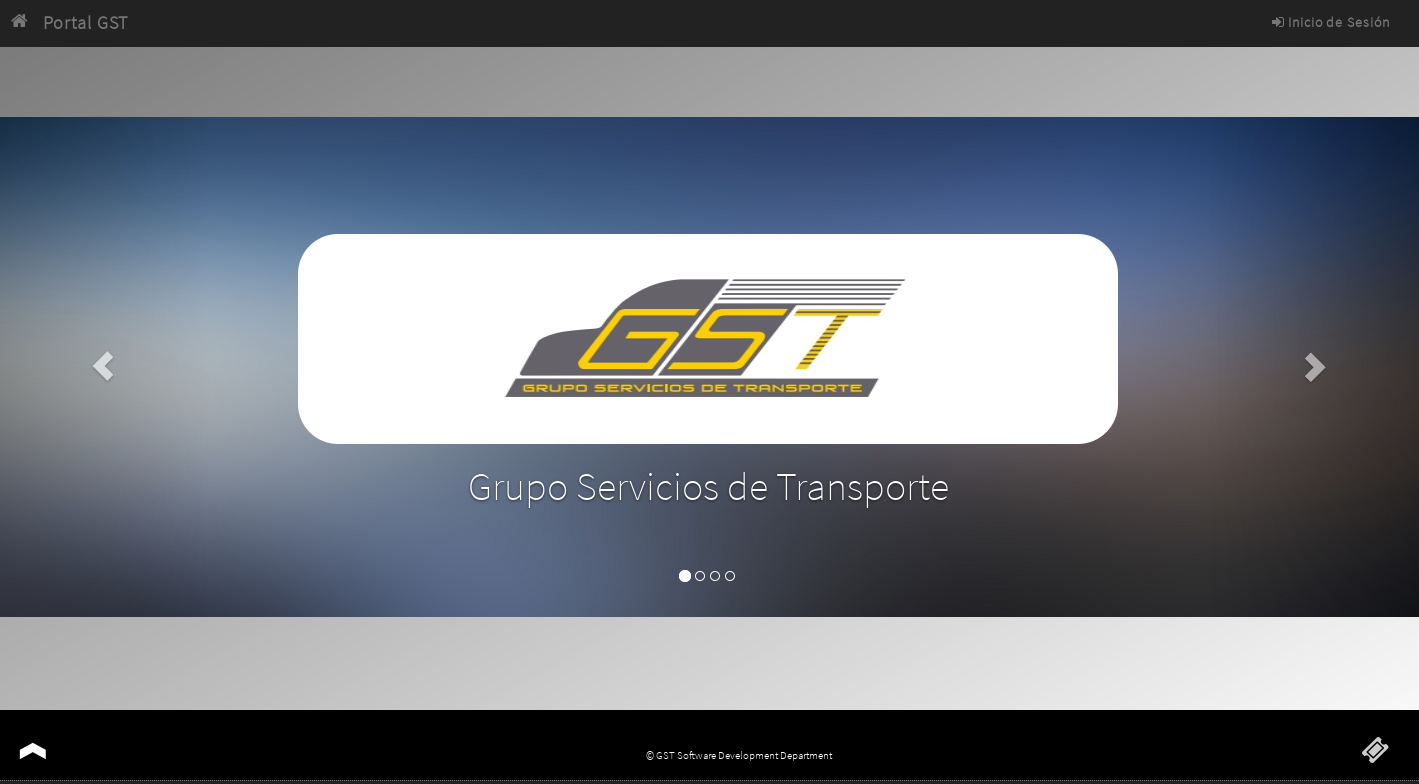
\includegraphics[angle=0,width=140mm,height=90mm]{img/Selection_064.png}
        \caption{landingPage}
        \label{sel064}
      \end{figure}

\newpage
    \subsubsection{Descripci\'on}
      La pantalla de \textbf{inicio} se divide en 3 Capas  Cinta Superior , Capa central , Cinta inferior
      en la Cinta Superior se encuentran Algunos controles y Menus , en la Capa Central consta de un Carrousel de Diapositivas
      en la Cinta inferior se encuentra un panel de control basico segun el modulo que se ejecute.

      \subsubsection{Descripcion de la pagina de inicio}
        \begin{figure}[htb]
          \centering
          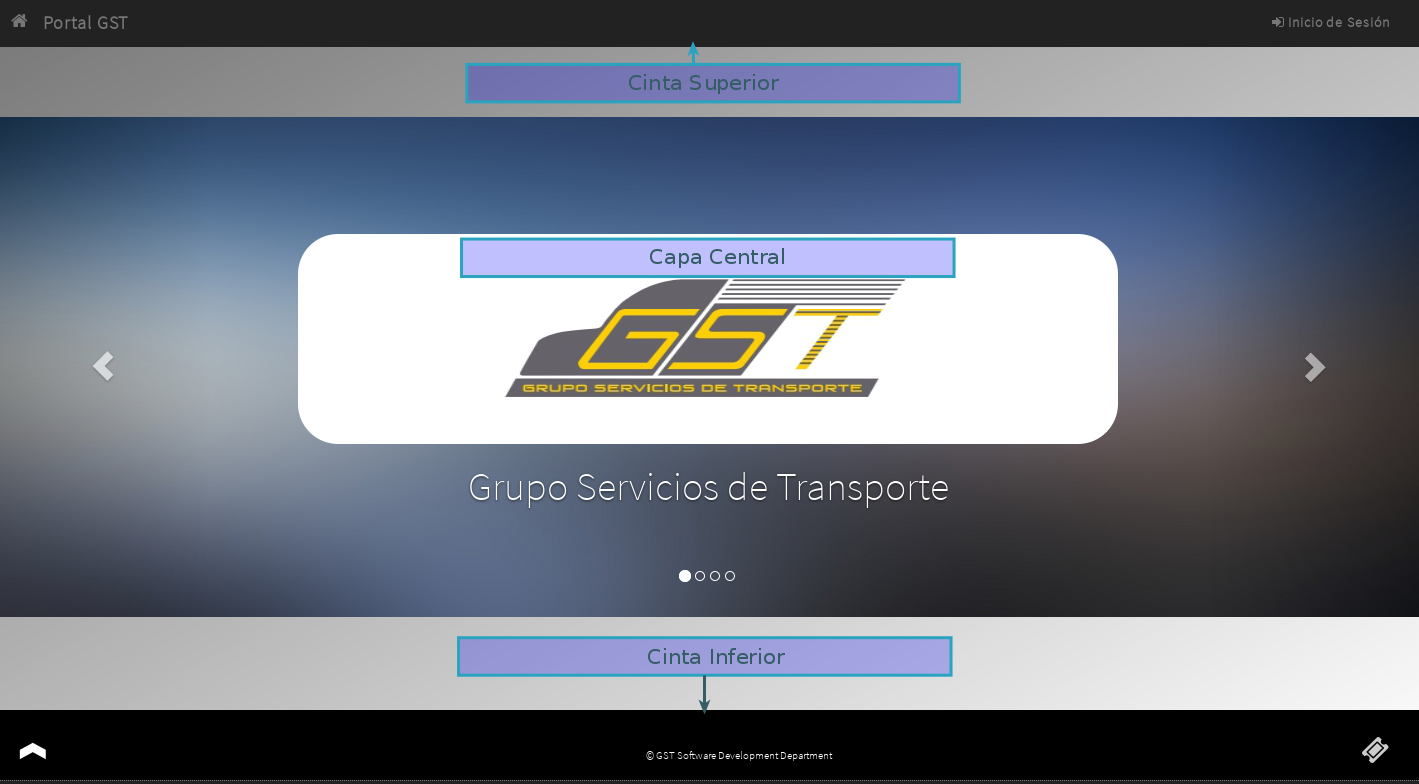
\includegraphics[angle=0,width=140mm,height=90mm]{img/Selection_064b.png}
          \caption{landingPage description}
          \label{sel064b}
        \end{figure}



    }
  \end{section}

\newpage
\begin{section}{\color{kblue}\sffamily{Document Viewer Module}}

	\begin{subsection}{\color{blackgreen}\sffamily{Overview of the Gst Group Policy's Module}}
	\sffamily
	{
    \subsubsection{Module Layouts}
      Para el Modulo de Politicas , se utiliza La cinta superior horizontal que contine el menu que clasifica las pol\'iticas del grupo Gst que al momento son tres :
      \subsubsection{Clasificacion del menu en la cinta superior horizontal:}
  			\begin{itemize}
  				\item[\ding{182}]
  				{
  					Politicas
  				}
  				\item[\ding{183}]
  				{
  					Manuales
  				}
  				\item[\ding{184}]
  				{
  					Procedimientos
  				}
  	   \end{itemize}

      y se muestran en la siguiente Imagen:

      \begin{figure}[htb]
        \centering
        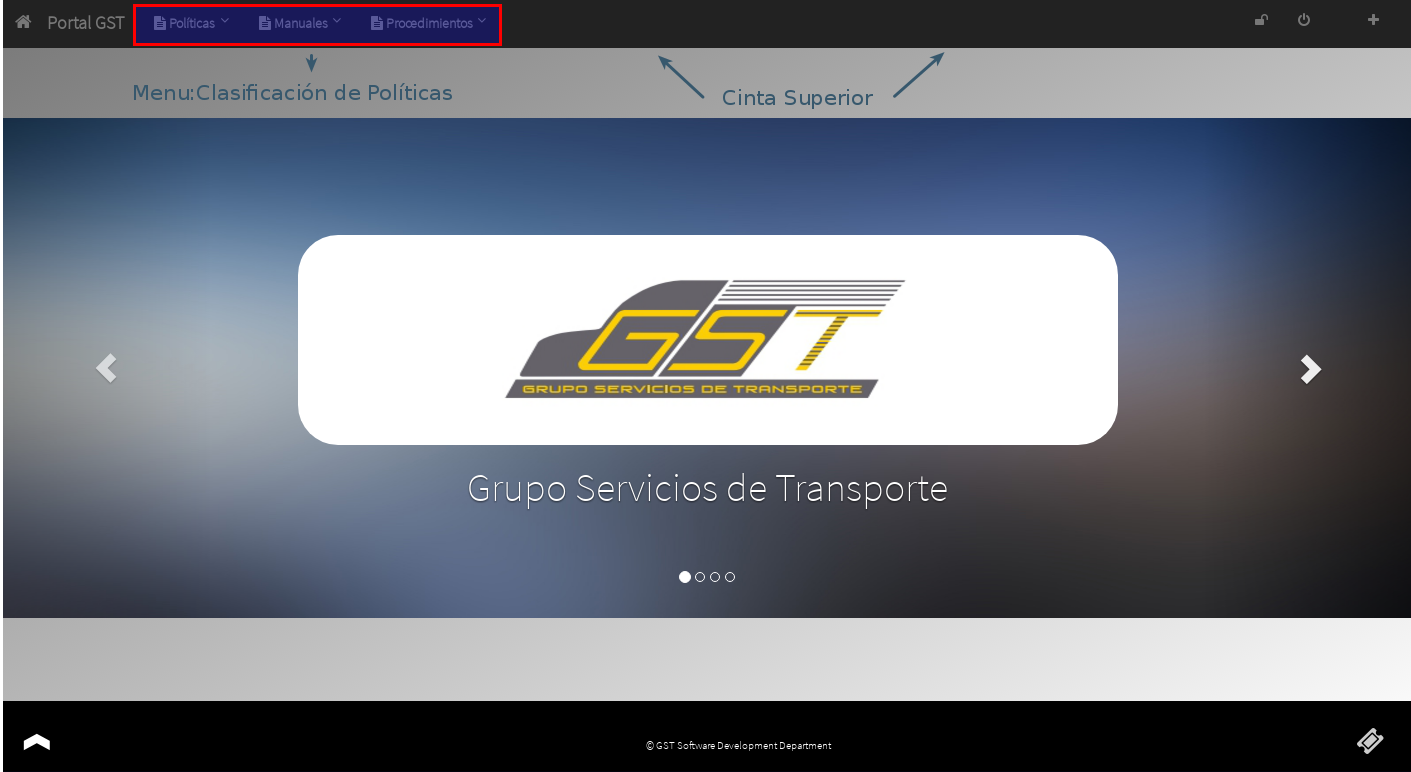
\includegraphics[angle=0,width=160mm,height=95mm]{img/Selection_037.png}
        \caption{Menu en la cinta superior}
        \label{menu}
      \end{figure}

\newpage
      Debajo de cada una se encuentran clasificados los departamentos del Grupo GST

      \subsubsection{Clasificacion del submenu : cinta horizontal}
        \begin{figure}[htb]
          \centering
          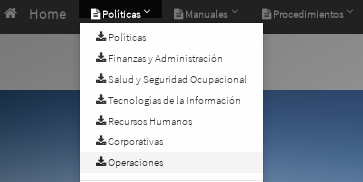
\includegraphics[angle=0,width=120mm,height=60mm]{img/Menu_034.png}
          \caption{Submenu : Categorias por Departamento}
          \label{sub_dept}
        \end{figure}


        \subsubsection{Clasificacion del submenu : cinta vertical}
          \begin{figure}[htb]
            \centering
            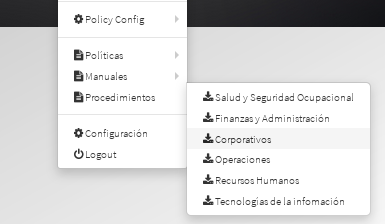
\includegraphics[angle=0,width=120mm,height=60mm]{img/Menu_053.png}
            \caption{Submenu : Categorias por Departamento}
            \label{sub_dept}
          \end{figure}


    En la Imagen se muestra el Submenu del Menu Polit\'icas si un Submenu no se encuentra disponible
    debera agregarse como sigue:
	}
	\end{section}

	% \newpage
	\sffamily
	{
	\begin{subsection}{\color{blackgreen}\sffamily{Add Items}}

	  \subsubsection{A\~nadir Submenu o Departamento:}
    Para agregar un Submenu o Departamento se tiene que tener acceso a las secciones de configuraci\'on del m\'odulo,
    que se encuentra en:
          \begin{lstlisting}[caption=Ruta Clasificador,style=customc]
            Policy Config \ Submenu-Clasifications
    			\end{lstlisting}


                \begin{figure}[htb]
                  \centering
                  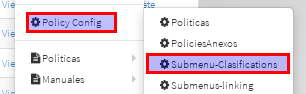
\includegraphics[angle=0,width=60mm,height=20mm]{img/Menu_036.png}
                  \caption{Ingresar a las opciones del Clasificador}
                  \label{class}
                \end{figure}

        Existen dos campos uno para agregar un clasificador y la otra para agregar el nombre que se mostrara en el submenu
        la funci\'on del campo \textquotedblleft{Clasificador}\textquotedblright es una descripci\'on que nos sirve para ligar el submenu al menu principal o ra\'iz

               \begin{figure}[htb]
                 \centering
                 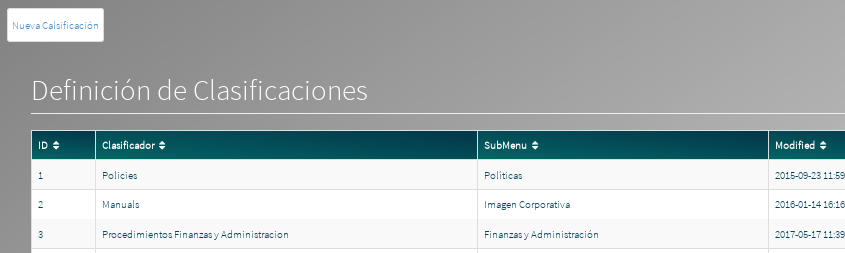
\includegraphics[angle=0,width=110mm,height=35mm]{img/Selection_035.png}
                 \caption{Seccion del Clasificador}
                 \label{class}
               \end{figure}

       En la parte superior derecha se encuentra el accesso para crear una Clasificaci\'on nueva \textquotedblleft Nueva Clasificaci\'on\textquotedblright
       y nos lleva al siguiente panel :
      \newpage
               \begin{figure}[htb]
                 \centering
                 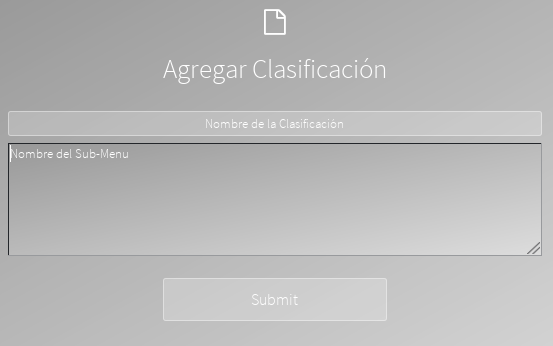
\includegraphics[angle=0,width=80mm,height=45mm]{img/Selection_038.png}
                 \caption{Panel Clasificación Nueva}
                 \label{class}
               \end{figure}

       Para crear una clasificaci\'on se debe definir un nombre identificador como clasificador y un nombre identificador como submenu
       por ejemplo si queremos agregar el submenu \textquotedblleft{Tecnolog\'ias de la Informaci\'on}\textquotedblright dentro de la categoria  \textquotedblleft{Procedimientos}\textquotedblright
               \begin{figure}[htb]
                 \centering
                 
\includegraphics[angle=0,width=43mm,height=28mm]{img/Menu_041.png}
                 \caption{Menu Procedimientos}
                 \label{add_subMenu}
               \end{figure}
       definimos el nombre Clasificador como \textquotedblleft{Procedimiento de las Tecnolog\'ias de la informaci\'on}\textquotedblright y el nombre submenu como \textquotedblleft{Tecnolog\'ias de la Informaci\'on}\textquotedblright
       este \'ultimo es el que se mostrara en el submenu debajo de \textquotedblleft{Procedimientos}\textquotedblright

              \begin{figure}[htb]
                \centering
                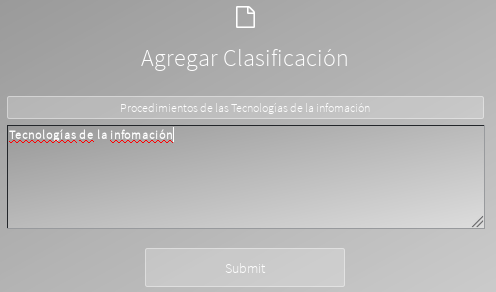
\includegraphics[angle=0,width=80mm,height=45mm]{img/Selection_042.png}
                \caption{Agregar Submenu}
                \label{add_submenu}
              \end{figure}

      \newpage
      Cuando se envia el registro , \'este aparecera normalmente en el \'ultimo registro con lo que podemos verificar que se ha agregado correctamente \\
            \begin{figure}[htb]
              \centering
              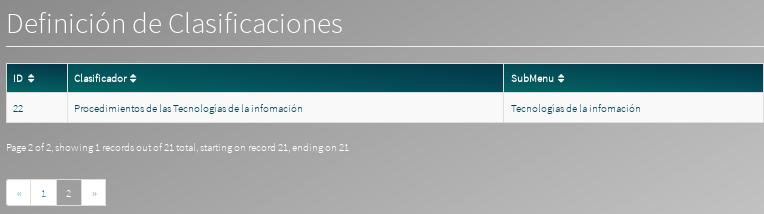
\includegraphics[angle=0,width=140mm,height=40mm]{img/Selection_043.png}
              \caption{Verificar el nuevo submenu}
              \label{add_submenu}
            \end{figure}

      Ahora esta clasificaci\'on debemos ligarla a la entrada \textquotedblleft{Procedimientos}\textquotedblright  en el Men\'u para que se agregue en la lista
            \begin{figure}[htb]
              \centering
              
\includegraphics[angle=0,width=43mm,height=35mm]{img/Menu_041.png}
              \caption{Lista de la Entrada Procedimientos}
              \label{add_subMenu}
            \end{figure}

% \newpage
      \subsubsection{Enganchar un Submenu con el Men\'u}

      Para ligar un submenu debemos ingresar a la secci\'on \textquotedblleft{submenu-hooks}\textquotedblright

        \begin{lstlisting}[caption=Ruta Ligar,style=customc]
          Policy Config \ Submenu-hooks
        \end{lstlisting}

              \begin{figure}[htb]
                \centering
                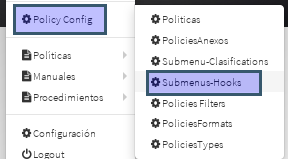
\includegraphics[angle=0,width=60mm,height=35mm]{img/Menu_044.png}
                \caption{Ingresar a las opciones de Enganche}
                \label{class}
              \end{figure}


      \newpage
      Y seleccionar la liga \textquotedblleft{New Hook}\textquotedblright  que nos llevara a
      la secci\'on de enganche donde podremos ligar una clasificaci\'on con alguna entrada del menu.
% Selection_047
              \begin{figure}[htb]
                \centering
                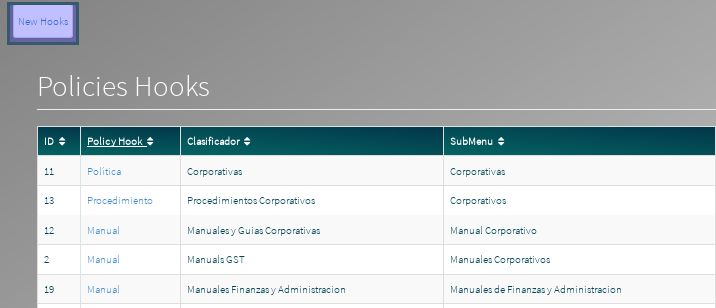
\includegraphics[angle=0,width=120mm,height=45mm]{img/Selection_047.png}
                \caption{Ingresar a las opciones de Enganche}
                \label{class}
              \end{figure}

      La secci\'on de Enganche nuevo \textquotedblleft{New Hook}\textquotedblright \\
      Consta de los siguientes :

              \subsubsection{Elementos para la configuraci\'on del Enganche:}

                \begin{figure}[htb]
                  \centering
                  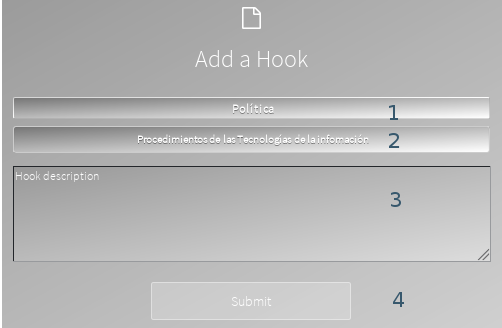
\includegraphics[angle=0,width=85mm,height=60mm]{img/Selection_048.png}
                  \caption{Ingresar a las opciones de Enganche}
                  \label{class}
                \end{figure}

          			\begin{itemize}
          				\item[\ding{182}]
          				{
          					Lista todos los elementos del Menu en la cinta horizontal superior
          				}
          				\item[\ding{183}]
          				{
          					Lista todos las Clasificaciones
          				}
          				\item[\ding{184}]
          				{
          					Descripci\'on que nos servira para indentificar el enganche
          				}
                  \item[\ding{185}]
          				{
          					Bot\'on para guardar la configuraci\'on
          				}
          	   \end{itemize}
\newpage
      Primero se selecciona a que entrada del menu va a pertenecer nuestra clasificaci\'on
          \begin{figure}[htb]
            \centering
            
\includegraphics[angle=0,width=75mm,height=7mm]{img/Menu_049.png}
            \caption{Seleccionamos la entrada o categor\'ia del menu}
            \label{cat}
          \end{figure}

      Despues buscamos la clasificaci\'on
          \begin{figure}[htb]
            \centering
            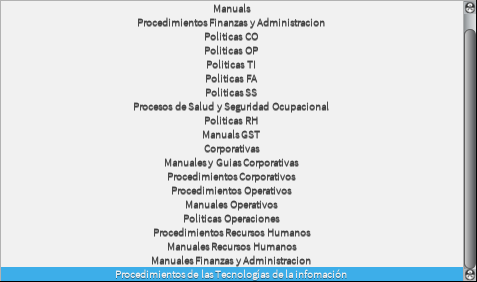
\includegraphics[angle=0,width=85mm,height=45mm]{img/Menu_050.png}
            \caption{Seleccionamos la Clasificaci\'on}
            \label{clt}
          \end{figure}

\newpage
      y por \'ultimo agregamos una descripci\'on y guardamos la informaci\'on
      con esto podemos ver que la clasificaci\'on \textbf{Procedimientos de las Tecnolog\'ias de la Informaci\'on} se a enganchado al elemento del menu \textbf{Procedimientos}
          \begin{figure}[htb]
            \centering
            
\includegraphics[angle=0,width=120mm,height=7mm]{img/Selection_051.png}
            \caption{Verificaci\'on del Enganche}
            \label{clta}
          \end{figure}

     Ahora podemos verificar en la cinta superior dentro del elemento \textbf{Procedimientos} la Clasificaci\'on \textbf{Procedimientos de las Tecnolog\'ias de la Informaci\'on}
         \begin{figure}[htb]
           \centering
           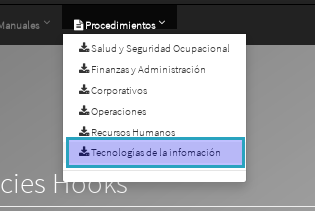
\includegraphics[angle=0,width=60mm,height=43mm]{img/Menu_052.png}
           \caption{Enganche correcto}
           \label{menu52}
         \end{figure}
	}
  \end{section}

	\begin{subsection}{\color{blackgreen}\sffamily{Add Document}}
	\sffamily
	{

      \subsubsection{Agregar Pol\'itica o Documento:}

      Para Agregar un Documento nuevo se ingresa a la secci\'on que se encuentra en :

      \begin{lstlisting}[caption=Ruta Documento,style=customc]
        Policy Config \ Documento
      \end{lstlisting}

        \begin{figure}[htb]
          \centering
          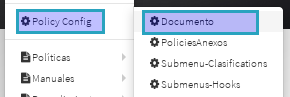
\includegraphics[angle=0,width=60mm,height=20mm]{img/Menu_054.png}
          \caption{Documento}
          \label{menu54}
        \end{figure}

      vamos a la liga \textbf{New Policy}
        \begin{figure}[htb]
          \centering
          
\includegraphics[angle=0,width=30mm,height=15mm]{img/Selection_055.png}
          \caption{Agregar Nuevo Documento}
          \label{sel55}
        \end{figure}
\newpage
      Los Campos son los Siguientes :

        \begin{figure}[htb]
          \centering
          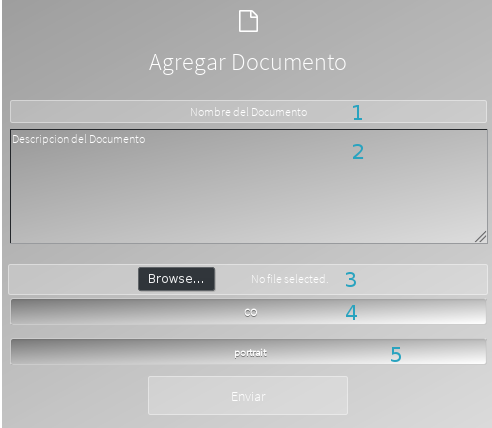
\includegraphics[angle=0,width=80mm,height=65mm]{img/Selection_056.png}
          \caption{Guardar Documento}
          \label{sel56}
        \end{figure}

        \begin{itemize}
          \item[\ding{182}]
          {
            Nombre del Documento
          }
          \item[\ding{183}]
          {
            Descripci\'on del Documento , este campo lo utiliza el motor de b\'usqueda , por lo tanto lo que se agregue en este campo impacta directamente con los patrones de b\'usqueda de los documentos
            aqu\'i se guardan las palabras clave que utiliza el motor de b\'usqueda , como ejemplo si el documento habla de vi\'aticos en los viajes , algunas palabras clave pueden ser : viajes ,vi\'aticos , boletos , etc
          }
          \item[\ding{184}]
          {
            Aqui se selecciona el Documento que se quiere guardar en el servidor
          }
          \item[\ding{185}]
          {
            Se elige la categoria a la que pertenecer\'a el documento en las cintas de men\'u por ejemplo si pertenece a la entrada \textbf{Procedimientos} , se debe seleccionar esta misma entrada
          }
          \item[\ding{186}]
          {
            Determina como se muestra la orientaci\'on del Documento \textbf{Portrait} : horizontal \\ \'o \textbf{landscape} : vertical
          }
          \item[\ding{187}]
          {
            Por \'ultimo se guarda y envia el Documento
          }
       \end{itemize}

       \newpage
       Una vez que el Documento esta en el servidor , se debe definir a que clasificaci\'on pertenece  para que se pueda mostrar adecuadamente,
       despues de guardar el documento
       \begin{figure}[htb]
         \centering
         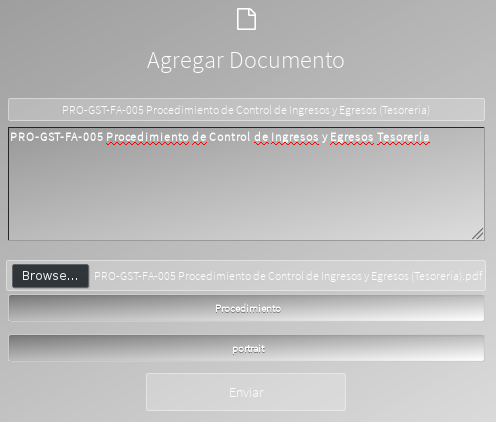
\includegraphics[angle=0,width=80mm,height=65mm]{img/Selection_057.png}
         \caption{Documento seleccionado}
         \label{sel57}
       \end{figure}

       automaticamente nos redirigira al listado de P\'oliticas y en \'esta pantalla debemos buscar el documento que acabamos de subir para indicarle
       en que clasificaci\'on queremos que se muestre.
       Por lo regular el documento que subimos se ordena hasta el final de la lista

         \begin{figure}[htb]
           \centering
           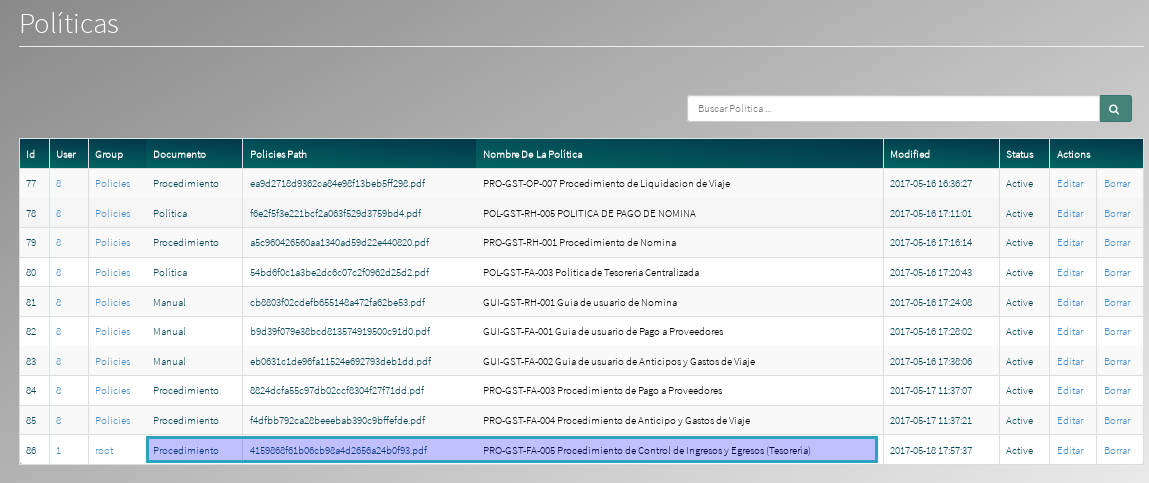
\includegraphics[angle=0,width=160mm,height=60mm]{img/Selection_059.png}
           \caption{listado de Pol\'iticas}
           \label{sel56}
         \end{figure}

\newpage
        Para indicar la clasificaci\'on seguimos la liga \textbf{Editar} y seleccionamos la Clasificacion que le corresponde :
        \begin{figure}[htb]
          \centering
          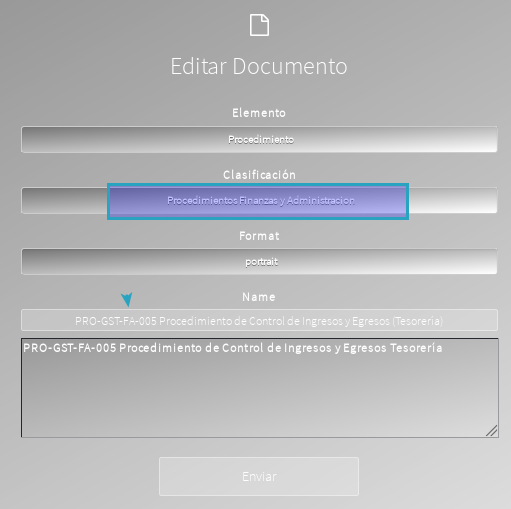
\includegraphics[angle=0,width=65mm,height=55mm]{img/Selection_060.png}
          \caption{Editar Clasificaci\'on}
          \label{sel60}
        \end{figure}

        Y comprobamos el cambio

        \begin{figure}[htb]
          \centering
          
\includegraphics[angle=0,width=30mm,height=25mm]{img/Menu_065.png}
          \caption{listar Menu}
          \label{sel56}
        \end{figure}

        \begin{figure}[htb]
          \centering
          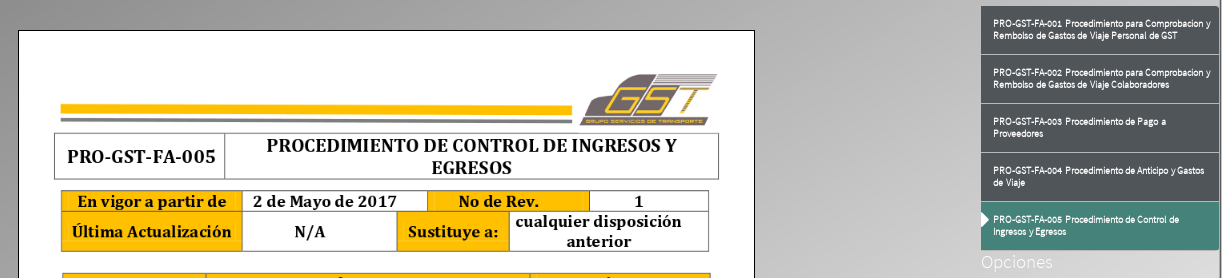
\includegraphics[angle=0,width=140mm,height=34mm]{img/Selection_063.png}
          \caption{Documento Actualizado}
          \label{sel63}
        \end{figure}
\newpage
        \subsubsection{Agregar Anexo:}

        Para anexar un documento para su descarga ligado a un Documento o Pol\'itica
        nos dirigimos a la siguiente ruta
        \begin{lstlisting}[caption=Ruta Anexo,style=customc]
          Policy Config \ Anexos
        \end{lstlisting}

        \begin{figure}[htb]
          \centering
          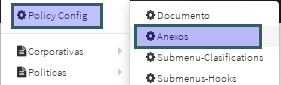
\includegraphics[angle=0,width=50mm,height=15mm]{img/Menu_066.png}
          \caption{Ruta Para Agregar un Documento anexo}
          \label{men66}
        \end{figure}

        La liga nos lleva a la secci\'on de \textbf{Anexos} tenemos el bot\'on de Anexo nuevo
        y un listado de los Documentos Anexos que existen en el servidor.

        \begin{figure}[htb]
          \centering
          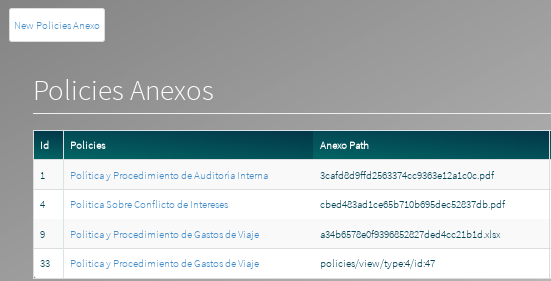
\includegraphics[angle=0,width=60mm,height=25mm]{img/Selection_067.png}
          \caption{listado de los Documentos anexos}
          \label{sel67}
        \end{figure}

        Para Agregar un nuevo documento seguimos la liga \texbf{New Policies Anexo} y en el panel agregamos los siguientes campos
        \begin{figure}[htb]
          \centering
          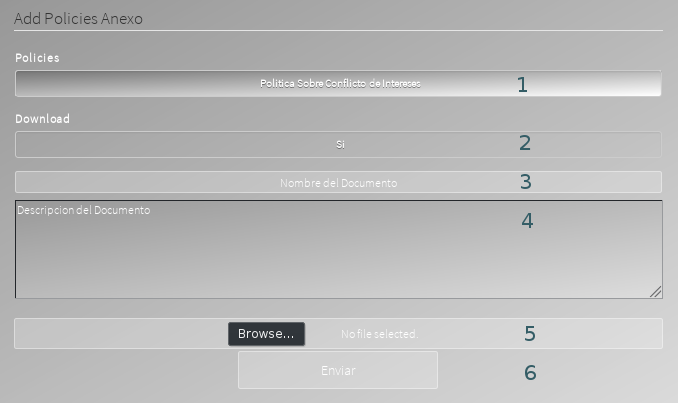
\includegraphics[angle=0,width=65mm,height=45mm]{img/Selection_068.png}
          \caption{Panel para agregar Documentos anexos}
          \label{sel68}
        \end{figure}

        \begin{itemize}
          \item[\ding{182}]
          {
            Seleccionamos la politica con la que vamos a ligar este anexo
          }
          \item[\ding{183}]
          {
            Definimos si el documento anexo sera descargable o no
          }
          \item[\ding{184}]
          {
            Definimos el nombre del documento anexo
          }
          \item[\ding{185}]
          {
            Definimos una descripci\'on
          }
          \item[\ding{186}]
          {
            Seleccionamos el documento anexo desde nuestro equipo o alg\'un recurso compartido
          }
          \item[\ding{187}]
          {
            Por \'ultimo se guarda y envia el Documento
          }
       \end{itemize}

       Al Guardar la configuraci\'on un icono aparece en la politica que seleccionamos al presionar.

       \begin{figure}[htb]
         \centering
         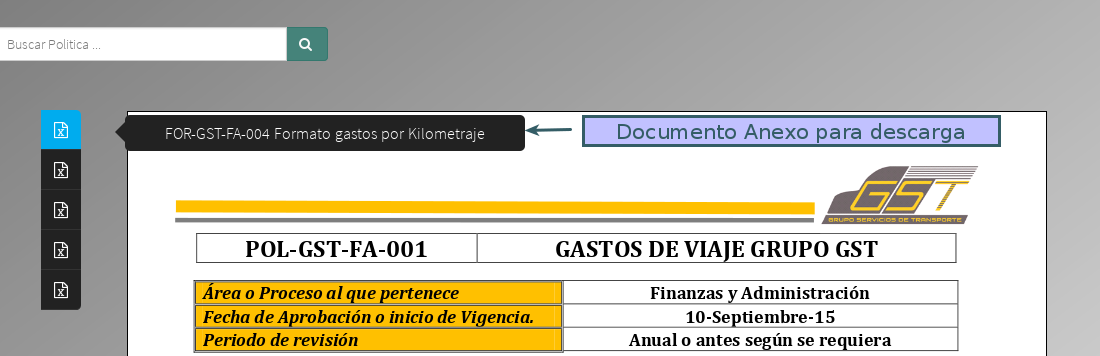
\includegraphics[angle=0,width=110mm,height=45mm]{img/Menu_069.png}
         \caption{Documento anexo}
         \label{men69}
       \end{figure}
	}
  \end{section}



%
% \newpage
%   \begin{section}{\color{kblue}\sffamily{Add Document}}
%   \sffamily
%   {
%
%   }
%   \end{section}



% FOR FOOTNOTES
  % \footnotesize{\scshape{}}

% FOR TABLES
% \begin{table}
% \end{table}

% EQUATIONS
% \begin{equation}
% 	costoLlamada = { totalDeMinutos x tarifa[codigoDePais] }
% 	\label{eq:costo de la llamada}
% \end{equation}
%
% \myequations{costo_call}

\end{document}
